\subsection{2.1 过程化SQL的块结构}
\begin{frame}[allowframebreaks,fragile]{2.1 过程化SQL的块结构}
    \begin{itemize}
        \item 过程化SQL 
        \begin{itemize} 
            \item SQL的扩展
            \item 增加了过程化语句功能
            \item 基本结构是块
            \begin{itemize} 
                \item 块之间可以互相嵌套
                \item 每个块完成一个逻辑操作
            \end{itemize}
        \end{itemize}
        \item 过程化SQL块的基本结构
        \begin{enumerate}
            \item 定义部分: DECLARE 变量、常量、游标、异常等   
            \begin{itemize}
                \item 定义的变量、常量等只能在该基本块中使用
                \item 当基本块执行结束时,定义就不再存在
            \end{itemize}
            \item 执行部分
\begin{block}{}
\begin{lstlisting}
BEGIN
    SQL语句、过程化SQL的流程控制语句
    EXCEPTION
    异常处理部分
END;
\end{lstlisting}
\end{block} 
\begin{itemize}
    \item 遇到不能继续执行的情况称为异常
    \item 在出现异常时,采取措施来纠正错误或报告错误
\end{itemize}
        \end{enumerate}
    \end{itemize}
\end{frame}

\subsection{变量和常量的定义}
\begin{frame}[allowframebreaks,fragile]{2.2 变量和常量的定义}
\begin{enumerate}
    \item 变量和常量的定义
    \begin{itemize}
        \item 变量名 数据类型 \lstinline{[[NOT NULL]:=初值表达式]}
        \item 变量名 数据类型 \lstinline{[[NOT NULL] 初值表达式]}
    \end{itemize}
    \item 常量定义
    \begin{itemize}
        \item 常量名 数据类型 \lstinline{CONSTANT :=常量表达式}
        \item 常量必须要赋予一个值,并且该值在存在期间或常量的作用域内不能改变。如果试图修改它,过程化SQL将返回一个异常
    \end{itemize}
    \item 赋值语句
    \begin{itemize}
    \item \lstinline{变量名称 :=表达式}
    \end{itemize}
\end{enumerate}
\end{frame}



\subsection{流程控制}
\begin{frame}[allowframebreaks,fragile]{2.3 流程控制}
\begin{itemize}
    \item 过程化SQL功能
    \begin{enumerate}
        \item 条件控制语句: IF-THEN,IF-THEN-ELSE和嵌套的IF语句 
        \begin{itemize}
            \item IF-THEN语句格式
            \item IF-THEN-ELSE语句格式
            \item 在THEN和ELSE子句中还可以再包含IF语句,即IF语句可以嵌套
        \end{itemize}
\begin{block}{}
\begin{lstlisting}
IF condition THEN
   Sequence_of_statements;        
END IF;   

IF condition THEN
   Sequence_of_statements1;  
ELSE
   Sequence_of_statements2;  
END IF;
\end{lstlisting}
\end{block} 
        
        \framebreak
        
        \item 循环控制语句: LOOP, WHILE-LOOP, FOR-LOOP

\begin{block}{}
\begin{lstlisting}
LOOP
  Sequence_of_statements;        
END LOOP;
\end{lstlisting}
\end{block} 
        \begin{itemize}
            \item 多数数据库服务器的过程化SQL都提供EXIT、BREAK或LEAVE等循环结束语句,保证LOOP语句块能够在适当的条件下提前结束
        \end{itemize}
\framebreak
\begin{block}{}
\begin{lstlisting}
WHILE condition LOOP
    Sequence_of_statements;
END LOOP;

\end{lstlisting}
\end{block} 

        \begin{itemize}
            \item 每次执行循环体语句之前,首先对条件进行求值
            \item 如果条件为真,则执行循环体内的语句序列
            \item 如果条件为假,则跳过循环并把控制传递给下一个语句
        \end{itemize}
\framebreak
\begin{block}{}
\begin{lstlisting}
FOR count IN [REVERSE] bound1 … bound2 LOOP
    Sequence_of_statements;
END LOOP;
\end{lstlisting}
\end{block} 

        \framebreak
        \item 错误处理 
        \begin{itemize}
            \item 如果过程化SQL在执行时出现异常,则应该让程序在产生异常的语句处停下来,根据异常的类型去执行异常处理语句 
            \item SQL标准对数据库服务器提供什么样的异常处理做出了建议,要求过程化SQL管理器提供完善的异常处理机制 
        \end{itemize}
    \end{enumerate}
\end{itemize}
\end{frame}



\subsection{游标的定义与使用}

\begin{frame}[allowframebreaks,fragile]{2.4 游标的定义与使用}
\begin{itemize}
    \item 游标
    \begin{itemize}
        \item 在过程化SQL中,如果\lstinline{SELECT}语句只返回一条记录,可以将该结果存放到变量中
        \item 当查询返回多条记录时,就要使用游标对结果集进行处理。一个游标与一个SQL语句相关联
        \item 游标的用户接口: 
        
        1.声明游标 2.打开游标 3.使用游标 4.关闭游标
    \end{itemize}    
        \framebreak
    \begin{enumerate}
        \item 声明游标
\begin{block}{}
\begin{lstlisting}
DECLARE 游标名 [(参数1 数据类型, 参数2 数据类型, …)] 
CURSOR FOR 
SELECT语句;
\end{lstlisting}
\end{block} 
        \begin{itemize}
            \item 定义游标仅仅是一条说明性语句,这时关系数据库管理系统并不执行\lstinline{SELECT}语句
        \end{itemize}
\framebreak
        
\item 打开游标
        
\begin{block}{}
\begin{lstlisting}
OPEN 游标名[(参数1 数据类型, 参数2 数据类型, …)];
\end{lstlisting}
\end{block} 
        \begin{itemize}
            \item 打开游标实际上是执行相应的\lstinline{SELECT}语句,把查询结果取到缓冲区中。这时游标处于活动状态,指针指向查询结果集中的第一条记录
        \end{itemize}
        \framebreak
\item 使用游标

\begin{block}{}
\begin{lstlisting}
FETCH 游标名 INTO 变量1[, 变量2,…];
\end{lstlisting}
\end{block} 
\begin{itemize}
    \item 变量必须与\lstinline{SELECT}语句中的目标列表达式一一对应
    \item 用FETCH语句把游标指针向前推进一条记录,同时将缓冲区中的当前记录取出来送至变量供过程化SQL进一步处理
    \item 循环执行FETCH语句,逐条取出结果集中的行进行处理
\end{itemize}

        \framebreak

\item 关闭游标
\begin{block}{}
\begin{lstlisting}
CLOSE 游标名;
\end{lstlisting}
\end{block} 
\begin{itemize}
    \item 游标被关闭后就不再和原来的查询结果集相联系
    \item 但被关闭的游标可以再次被打开,与新的查询结果相联系
\end{itemize}





    \end{enumerate}
\end{itemize}
\end{frame}
 
\begin{frame}[fragile]{2.4 游标的定义和使用(例)}
\begin{itemize}
    \item 根据给定学号20180001,使用游标输出该学生的全部选课记录
\begin{block}{}
\begin{lstlisting}[xleftmargin=0.1\textwidth,linewidth=\textwidth]
DECLARE
    CnoOfStudent CHAR(10);
    GradeOfStudent INT;
    mycursor CURSOR FOR 
    SELECT Cno,Grade FROM SC WHERE Sno = '20180001';
BEGIN
    OPEN mycursor;      /*打开游标*/
    LOOP                /*循环遍历游标*/ 
        FETCH mycursor INTO CnoOfStudent, GradeOfStudent; /*检索游标*/
        EXIT WHEN mycursor \%NOTFOUND;
        RAISE NOTICE 'Sno:20180001, Cno:\%, Grade:\%', CnoOfStudent, GradeOfStudent;
    END LOOP;
    CLOSE mycursor;     /*关闭游标*/
END;
\end{lstlisting}
\end{block} 
\end{itemize}
\end{frame}


\subsection{存储过程}
\begin{frame}[allowframebreaks,fragile]{存储过程}
\begin{itemize}
    \item 存储过程
    \begin{itemize}
        \item 类似于高级语言程序,过程化SQL程序也可以被命名和编译,并保存在数据库中,称为存储过程(stored procedure)或存储函数(stored function),供其他过程化SQL调用
        \item 存储过程或存储函数也是一类数据库的对象,需要有创建、删除等语句。这里的存储函数指自定义函数
    \end{itemize}
    \item 存储过程的用户接口
    \begin{enumerate}
        \item 创建存储过程
        \item 执行存储过程 
        \item 修改存储过程
        \item 删除存储过程 
    \end{enumerate}
\end{itemize}
\end{frame}

\begin{frame}[allowframebreaks,fragile]{存储过程-创建存储过程}
\begin{enumerate}
    \item 创建存储过程
\begin{block}{}
\begin{lstlisting}[linewidth=\textwidth]
CREATE OR REPLACE PROCEDURE过程名(
    [[IN|OUT|INOUT] 参数1 数据类型,
    [IN|OUT|INOUT] 参数2 数据类型,
    …]
)                       /*存储过程首部*/ 
AS <过程化SQL块>;       /*存储过程体,描述该存储过程的操作*/
\end{lstlisting}
\end{block} 
\begin{itemize}
    \item 过程名:数据库服务器合法的对象标识
    \item 参数列表:存储过程提供了 IN、OUT、INOUT 三种参数模式,分别对应输入、输出、输入输出三种语义,不声明参数模式时,缺省为 IN 类型。输入参数在被调用时需要指定参数值,输出参数调用时不传入参数值,而是作为返回值返回。输入输出参数调用时需要传入初始值,并会返回操作后的最终值。参数列表中需要指定参数模式、参数名、以及参数的数据类型
    \item 过程体:是一个<过程化SQL块>,包括声明部分和可执行语句部分 
\end{itemize}
\end{enumerate}
\framebreak
\end{frame}

\begin{frame}[fragile]{存储过程-创建存储过程}
\begin{itemize}
    \item 给定学生学号,计算学生的平均学分绩点GPA
    \item 求解思路
    \begin{itemize}
        \item 给定学生学号,找出该学生所有选修课程的学分、成绩
        \item 根据每门课程的成绩,参照成绩和绩点对照表,确定该成绩所处的范围,找出该门课程对应的学分绩点
    \end{itemize}
       \begin{figure}
        \centering
        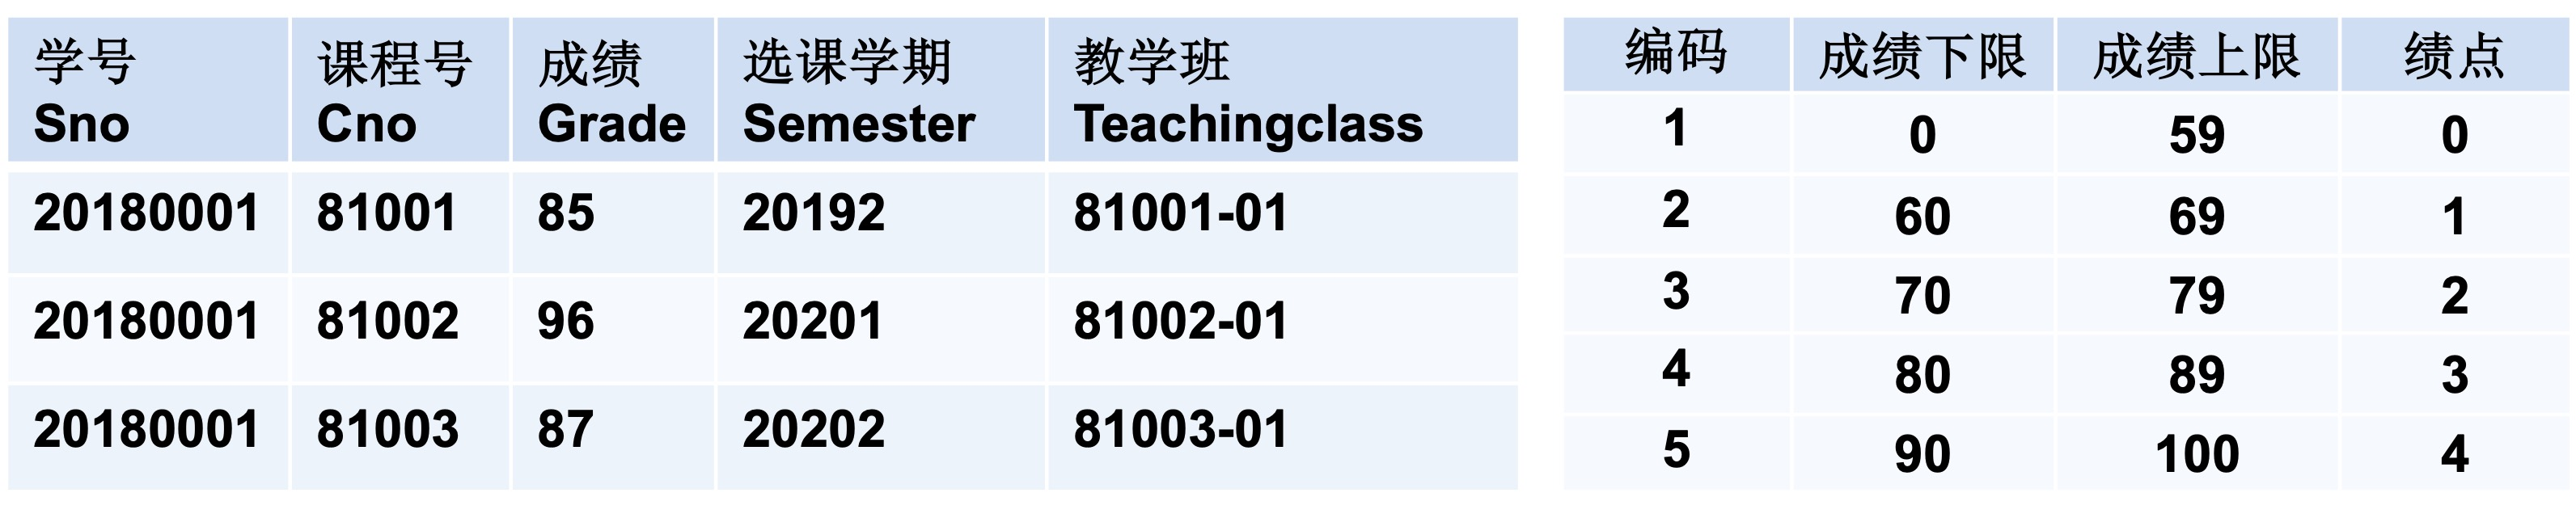
\includegraphics[width=0.8\textwidth]{figure/fig-9.jpg}
    \end{figure}

\end{itemize}
\end{frame}

\begin{frame}[fragile]{存储过程-创建存储过程}
\begin{itemize}
    \item 给定学生学号,计算学生的平均学分绩点GPA
    \item 求解思路
    \begin{itemize}
        \item “81001”课程考试成绩为85分,参照右下表,85分对应成绩范围为[80,89],该门课程对应的学分绩点为3。类似地,课程号为“81002”对应的学分绩点为4, 课程号为“81003”对应的学分绩点为3
        \item 81001-81003三门课程的学分都是4。根据平均学分绩点GPA的计算公式=总学分绩/总学分=(每门课程的学分*对应课程的绩点)的总和/12 = (3*4 + 4*4 + 3*4)/12 = 3.33	
    \end{itemize}
       \begin{figure}
        \centering
        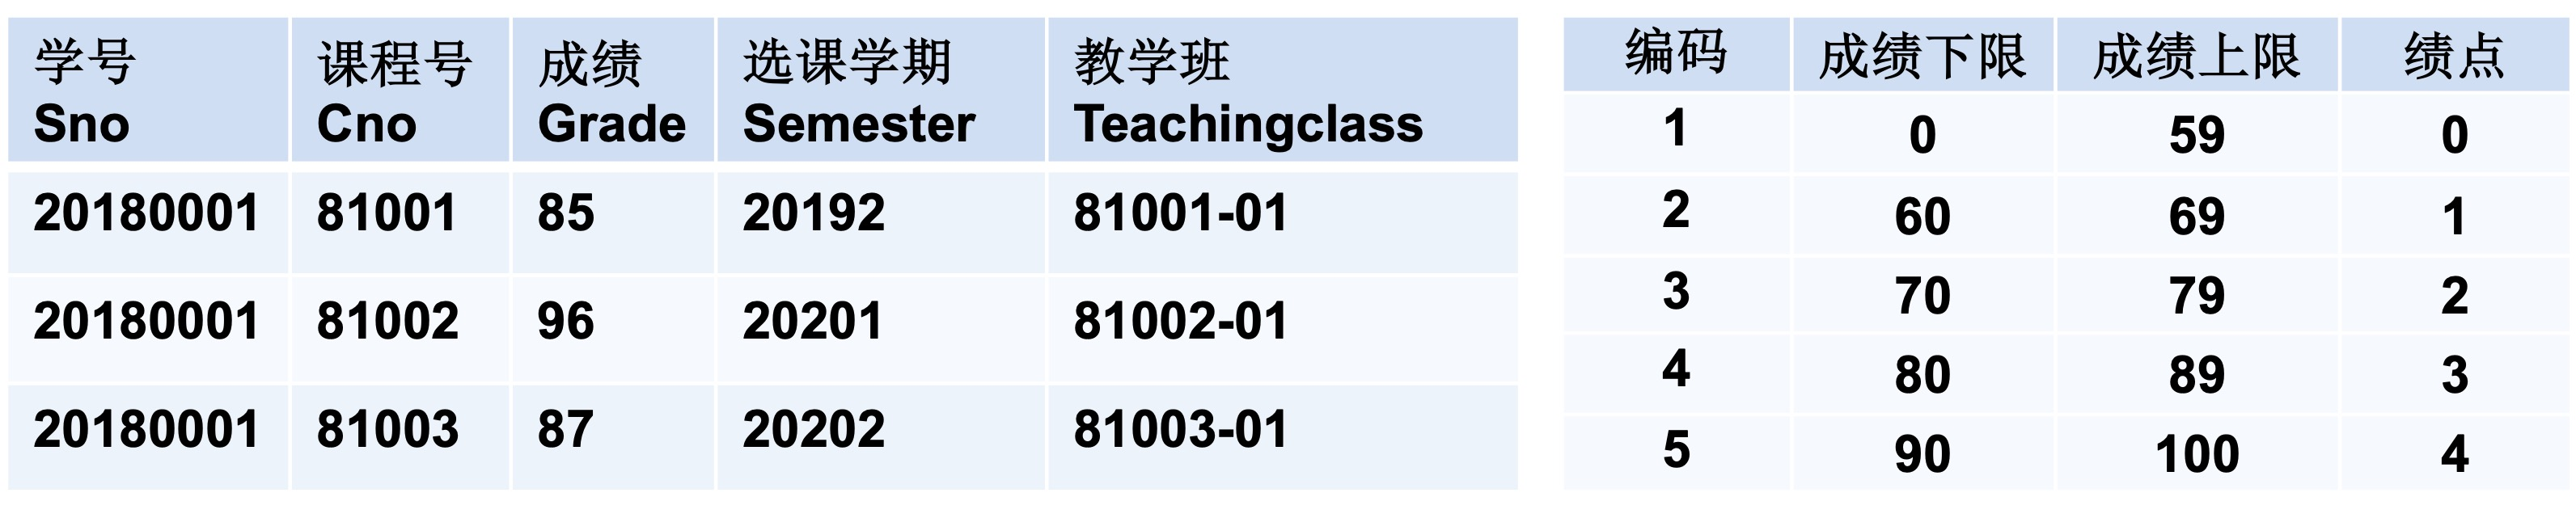
\includegraphics[width=0.8\textwidth]{figure/fig-9.jpg}
    \end{figure}
\end{itemize}
\end{frame}

\begin{frame}[fragile,allowframebreaks]{存储过程-创建存储过程}
\begin{itemize}
    \item 给定学生学号,计算学生的平均学分绩点GPA
\end{itemize}
\begin{block}{}
\begin{lstlisting}[linewidth=\textwidth]
CREATE OR REPLACE PROCEDURE compGPA(      /*定义存储过compGPA*/
    IN inSno CHAR(10),     /*输入参数:学生学号inSno*/
    OUT outGPA FLOAT)      /*输出参数:平均学分绩outGPA*/
    AS 
    DECLARE
        courseGPA INT;     /*声明变量courseGPA,临时存储课程学分绩 */
        totalGPA INT;      /*声明变量totalGPA,临时存储总学分绩 */
        totalCredit INT;   /*声明变量totalCredit,临时存储总学分*/
        grade INT;         /*声明变量grade,临时存储学生成绩 */
        credit INT;         /*声明变量credit ,临时存储课程学分 */
        mycursor CURSOR FOR         /*声明游标mycursor */ 
        SELECT Ccredit, grade FROM SC, Course 
        WHERE Sno = inSno AND SC.Cno = Course.Cno;   
\end{lstlisting}
\end{block}
\framebreak
\begin{block}{}
\begin{lstlisting}[firstnumber=15,linewidth=\textwidth]
    BEGIN 
        totalGPA := 0;
        totalCredit := 0;
        OPEN mycursor;             /*打开游标mycursor */
        LOOP                             /*循环遍历游标*/
            FETCH mycursor INTO credit, grade;     /*检索游标*/
            EXIT WHEN mycursor%NOTFOUND;
            IF grade BETWEEN 90 AND 100 THEN courseGPA := 4.0; 
            ELSIF grade BETWEEN 80 AND 89 THEN courseGPA := 3.0; 
            ELSIF grade BETWEEN 70 AND 72 THEN courseGPA := 2.0; 
            ELSIF grade BETWEEN 60 AND 69 THEN courseGPA := 1.0; 
            ELSE courseGPA := 0; 
            END IF;   /*参照表8.2,根据成绩找出某门课程对应的学分绩点*/
                    totalGPA := totalGPA + courseGPA * credit;
            totalCredit := totalCredit + credit;
        END LOOP;
        CLOSE mycursor;            /*关闭游标mycursor */
        outGPA:= 1.0 * totalGPA / totalCredit;
    END;
\end{lstlisting}
\end{block}

\end{frame}


\begin{frame}[allowframebreaks,fragile]{存储过程}
\begin{enumerate}
\setcounter{enumi}{1}
    \item 执行存储过程

\begin{block}{}
\begin{lstlisting}    
CALL/PERFORM  [PROCEDURE] 过程名([参数1,参数2,...]);
\end{lstlisting}
\end{block}
\begin{itemize}
    \item 使用CALL或者PERFORM等方式激活存储过程的执行
    \item 在过程化SQL中,数据库服务器支持在过程体中调用其他存储过程
\end{itemize}
\end{enumerate}

\framebreak
\begin{itemize}
    \item 查询学号为“20180001”学生的课程GPA。
    \begin{itemize}
        \item 在调用含有输入参数和输入输出参数的存储过程时,需要指定具体的参数值。在调用含有输出参数的存储过程时,对应位置不需要传入参数值,但需要事先定义输出变量
    \end{itemize}
\end{itemize}

\begin{block}{}
\begin{lstlisting}
DECLARE outGPA FLOAT;
BEGIN
    CALL compGPA('20180001',outGPA);
    RAISE NOTICE 'GPA: %', outGPA;
END;

\end{lstlisting}
\end{block}

\end{frame}

\begin{frame}[allowframebreaks,fragile]{存储过程}
\begin{enumerate}
\setcounter{enumi}{2}
    \item 修改存储过程
    \begin{itemize}
        \item 重命名/重新编译
\begin{block}{}
\begin{lstlisting}
ALTER PROCEDURE 过程名1  RENAME TO 过程名2;
ALTER PROCEDURE 过程名1 COMPILE;
\end{lstlisting}
\end{block}
    \end{itemize}
    \item 删除存储过程 
\begin{block}{}
\begin{lstlisting}
DROP  PROCEDURE 过程名;
\end{lstlisting}
\end{block}

\end{enumerate}
\end{frame}


\begin{frame}[allowframebreaks,fragile]{存储过程}
\begin{itemize}
    \item 存储过程的优点
    \begin{enumerate}
\item 运行效率高
\item 降低了客户机和服务器之间的通信量	
\item 方便实施企业规则
\end{enumerate}
\end{itemize}
\end{frame}

\subsection{存储函数}
\begin{frame}[allowframebreaks,fragile]{存储函数}
\begin{itemize}
    \item 存储函数和存储过程的异同
    \begin{enumerate}
\item 同: 都是持久性存储模块
\item 异:函数必须指定返回的类型
\end{enumerate}
\end{itemize}
\end{frame}

\begin{frame}[allowframebreaks,fragile]{存储函数}
\begin{enumerate}
    \item 函数的定义/执行/修改语句 
\begin{block}{}
\begin{lstlisting}
CREATE OR REPLACE FUNCTION 函数名([参数1 数据类型, 参数2数据类型, ...]) 
RETURNS <类型>
AS  <过程化SQL块>;

CALL/SELECT 函数名 ([参数1,参数2,…]);

ALTER FUNCTION 函数名1 RENAME TO 函数名2;
ALTER FUNCTION 函数名 COMPILE;

\end{lstlisting}
\end{block}

\end{enumerate}

\end{frame}



